\begin{enumerate}
	\item [(الف)]
	جدول درستی مدار به‌صورت زیر به‌دست می‌آید:
	
	
	\begin{latin}
		\[
		\begin{array}{|c|c|c|c|c|c|c|c|c|}
			\hline
			IN_1 & IN_2 & IN_3 & IN_4 & OUT_1 & OUT_2 & OUT_3 & OUT_4 \\
			\hline\hline
			0 & 0 & 0 & 0 & 0 & 0 & 0 & 0 \\
			0 & 0 & 0 & 1 & 0 & 0 & 0 & 0 \\
			0 & 0 & 1 & 0 & 0 & 0 & 0 & 0 \\
			0 & 0 & 1 & 1 & 0 & 0 & 0 & 0 \\
			0 & 1 & 0 & 0 & 0 & 0 & 0 & 0 \\
			0 & 1 & 0 & 1 & 0 & 0 & 1 & 0 \\
			0 & 1 & 1 & 0 & 0 & 1 & 0 & 0 \\
			0 & 1 & 1 & 1 & 0 & 1 & 1 & 0 \\
			1 & 0 & 0 & 0 & 0 & 0 & 0 & 0 \\ 
			1 & 0 & 0 & 1 & 1 & 1 & 0 & 0 \\
			1 & 0 & 1 & 0 & 0 & 0 & 0 & 0 \\
			1 & 0 & 1 & 1 & 1 & 1 & 0 & 0 \\
			1 & 1 & 0 & 0 & 0 & 0 & 0 & 0 \\
			1 & 1 & 0 & 1 & 1 & 1 & 1 & 0 \\
			1 & 1 & 1 & 0 & 0 & 1 & 0 & 0 \\
			1 & 1 & 1 & 1 & 1 & 0 & 0 & 1 \\
			\hline
		\end{array}
		\]
	\end{latin}
	
	
	
	
	\item [(ب)]
	جداول کارنو برای چهار خروجی به‌صورت زیر می‌شود:
	
	\begin{latin}
		\begin{minipage}{0.48\textwidth}
			\centering
			\begin{karnaugh-map}[4][4][1][$IN_2$][$IN_1$][$IN_4$][$IN_3$](label=corner)
				\maxterms{0,1,2,3,4,5,8,9,10,11,12,13}
				\implicant{0}{9}
				\implicantedge{0}{2}{8}{10}
			\end{karnaugh-map}
			\caption{K-Map 1}
			$OUT_1=IN_4 \cdot IN_1$
		\end{minipage}
		\hfill
		\begin{minipage}{0.48\textwidth}
			\centering
			\begin{karnaugh-map}[4][4][1][$IN_2$][$IN_1$][$IN_4$][$IN_3$](label=corner)
				\maxterms{0,1,2,3,4,5,8,10,12,15}
				\implicant{0}{8}
				\implicant{0}{2}
				\implicant{0}{5}
				\implicant{15}{15}
				\implicantcorner
			\end{karnaugh-map}
			\caption{K-Map 1}
			$OUT_2=(IN_3 + IN_4) \cdot (IN_1 + IN_2) \cdot (IN_2 + IN_4) \cdot (IN_1'+IN_2'+IN_3'+IN_4')$
		\end{minipage}	
	\end{latin}
	
	
	
	
	
	
	
	
	\begin{latin}
		\begin{minipage}{0.48\textwidth}
			\centering
			\begin{karnaugh-map}[4][4][1][$IN_2$][$IN_1$][$IN_4$][$IN_3$](label=corner)
				\maxterms{0,1,2,3,4,6,8,9,10,11,12,14,15}
				\implicantedge{0}{2}{8}{10}
				\implicantedge{0}{8}{2}{10}
			\end{karnaugh-map}
			\caption{K-Map 1}
			$OUT_3=IN_4 \cdot IN_2$
		\end{minipage}
		\hfill
		\begin{minipage}{0.48\textwidth}
			\centering
			\begin{karnaugh-map}[4][4][1][$IN_2$][$IN_1$][$IN_4$][$IN_3$](label=corner)
				\maxterms{0,1,2,3,4,5,6,7,8,9,10,11,12,13,14}
				\implicant{0}{9}
				\implicant{0}{6}
				\implicantedge{0}{8}{2}{10}
				\implicantedge{0}{2}{8}{10}
			\end{karnaugh-map}
			\caption{K-Map 1}
			$OUT_4=IN_1 \cdot IN_2 \cdot IN_3 \cdot IN_4$
		\end{minipage}	
	\end{latin}
	
	همچنین مدار ساده شده به‌صورت زیر رسم می‌شود:
	
	\begin{figure}[h]
		\centering
		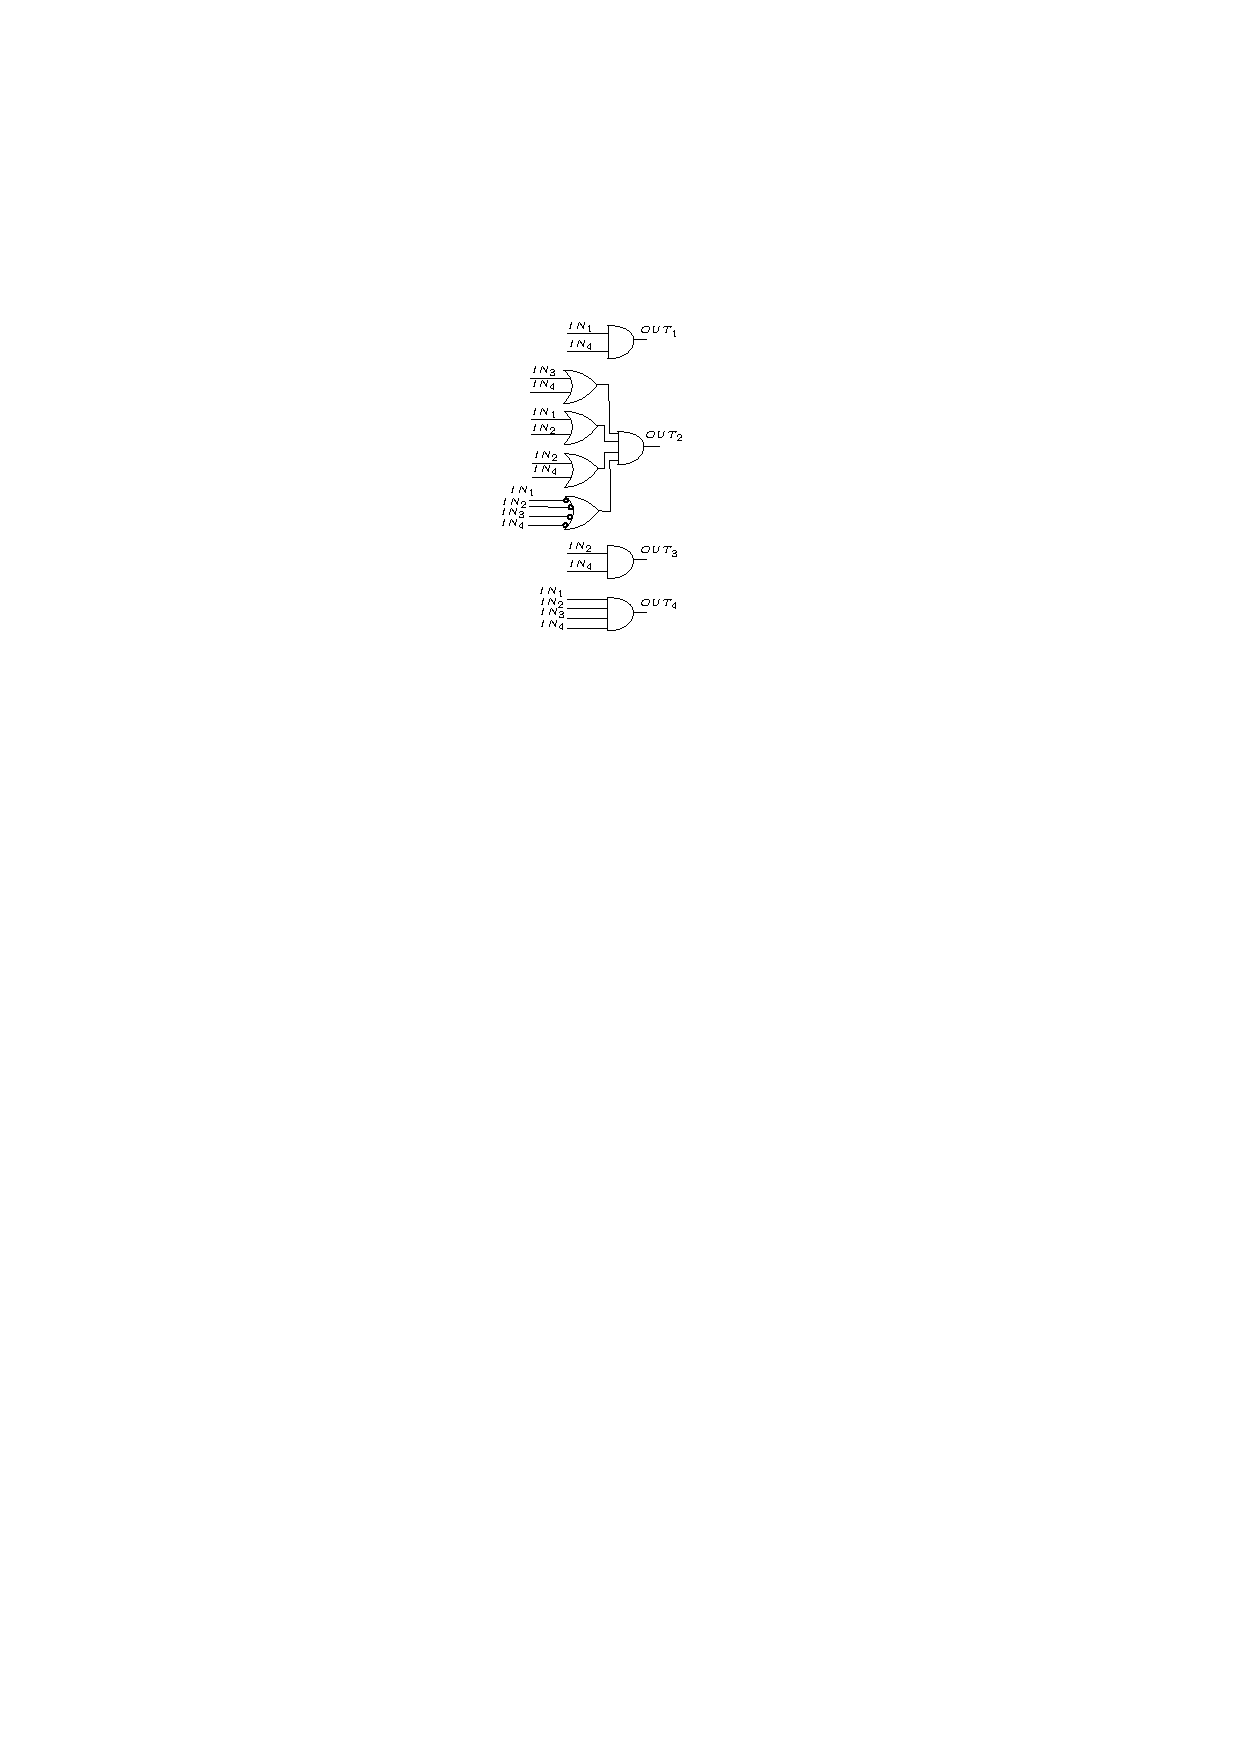
\includegraphics[width=0.5\textwidth]{fig/Q3_circ_new.pdf}
		\caption{مدار ساده شده}
		\label{Q3circ}
	\end{figure}
	
	
	
\end{enumerate}

